%%%%%%%%%%%%%%%%%%%%%%%%%%%%%%%%%%%%%%%%%
% University Assignment Title Page 
% LaTeX Template
% Version 1.0 (27/12/12)
%
% This template has been downloaded from:
% http://www.LaTeXTemplates.com
%
% Original author:
% WikiBooks (http://en.wikibooks.org/wiki/LaTeX/Title_Creation)
%
% License:
% CC BY-NC-SA 3.0 (http://creativecommons.org/licenses/by-nc-sa/3.0/)
% 
% Instructions for using this template:
% This title page is capable of being compiled as is. This is not useful for 
% including it in another document. To do this, you have two options: 
%
% 1) Copy/paste everything between \begin{document} and \end{document} 
% starting at \begin{titlepage} and paste this into another LaTeX file where you 
% want your title page.
% OR
% 2) Remove everything outside the \begin{titlepage} and \end{titlepage} and 
% move this file to the same directory as the LaTeX file you wish to add it to. 
% Then add \input{./title_page_1.tex} to your LaTeX file where you want your
% title page.
%
%%%%%%%%%%%%%%%%%%%%%%%%%%%%%%%%%%%%%%%%%
%\title{Title page with logo}
%----------------------------------------------------------------------------------------
%	PACKAGES AND OTHER DOCUMENT CONFIGURATIONS
%----------------------------------------------------------------------------------------

\documentclass[12pt]{article}

\usepackage[francais]{babel}
\usepackage[utf8x]{inputenc}
\usepackage[T1]{fontenc}
\usepackage{color}

\usepackage{amsmath}
\usepackage{graphicx}
\usepackage{enumerate}
\usepackage{url}
\usepackage{caption}

% Define new command
\newcommand{\HRule}{\rule{\linewidth}{0.5mm}}

\newcommand{\crt}{\emph{Nexys 4 DDR\ }}
%\def\thesubsection{\alph{section}}

\begin{document}

\begin{titlepage}

\center % Center everything on the page
 
%----------------------------------------------------------------------------------------
%	HEADING SECTIONS
%----------------------------------------------------------------------------------------

\textsc{\LARGE Universit\'e Pierre et Marie Curie}\\[1.5cm] % Name of your university/college
\textsc{\Large PSESI}\\[0.5cm] % Major heading such as course name

%----------------------------------------------------------------------------------------
%	TITLE SECTION
%----------------------------------------------------------------------------------------

\HRule \\[0.4cm]
{ \huge \bfseries Rapport de pr\'e-soutenance}\\[0.4cm] % Title of your document
{ \huge \bfseries D\'eveloppement sur FPGA \\d'un système d'aiguillage
  \\pour centrale DCC sur train miniature}\\[0.4cm] % Title of your document
\HRule \\[1.5cm]
 
%----------------------------------------------------------------------------------------
%	AUTHOR SECTION
%----------------------------------------------------------------------------------------

\begin{minipage}{0.4\textwidth}
\begin{flushleft} \large
\emph{\'Etudiant:}\\
Maxime \textsc{AYRAULT} 3203694 % Your name
\end{flushleft}
\end{minipage}
~
\begin{minipage}{0.4\textwidth}
\begin{flushright} \large
\emph{Encadrant:} \\
Julien \textsc{DENOULET} % Supervisor's Name
\end{flushright}
\end{minipage}\\[2cm]

%----------------------------------------------------------------------------------------
%	DATE SECTION
%----------------------------------------------------------------------------------------

{\large \today}\\[2cm] % Date, change the \today to a set date if you want to be precise

%----------------------------------------------------------------------------------------
%	LOGO SECTION
%----------------------------------------------------------------------------------------

%%\begin{figure}
%%  \subfigure[]{
\includegraphics[scale=0.2\textwidth]{logo.png}} 
%%\end{figure} 

\includegraphics[width=0.2\textwidth]{logo.png}

%----------------------------------------------------------------------------------------

\vfill % Fill the rest of the page with whitespace

\end{titlepage}



%\begin{abstract}
%Your abstract here.
%\end{abstract}

\section{Introduction}
\label{sec:introduction}

\subsection{\underline{Contexte et encadrement}}

Depuis plusieurs ann\'ees, la plateforme d'ingénierie de l'UPMC d\'eveloppe un projet de
gestion de maquettes de trains. Ce projet se base sur une
\emph{centrale DCC}. Cette centrale permet de recevoir la position des
trains et des aiguilles et d'envoyer des commandes en utilisant le
\emph{protocole DCC}.

Ce projet est r\'ealis\'e seul et est encadr\'e par M. Denoulet. Ce projet se d\'eroule sur une dur\'ee de 6 semaines.
Il est r\'ealis\'e dans le cadre d'un projet SESI.

\subsection{\underline{Objectifs}}

L'objectif du projet consiste, dans un premier temps, à porter la
\emph{centrale DCC} implement\'ee par d'autres \'etudiants sur une nouvelle
carte mat\'eriel \emph{FPGA}. La version courante de la centrale tourne sur
une carte \emph{Spartan 6}, elle est remplac\'ee par notre \crt qui est
une carte plus r\'ecente et possède une interface plus complète
\emph{(switchs, boutons, afficheurs 7 segments...)}
Dans un second temps, le projet consiste à ajouter la commande en
sécurité des aiguillages.

Je propose de commencer par une gestion manuelle des aiguillages avec
les diff\'erents switchs de la carte sans v\'erification de
s\'ecurit\'e.
Puis une fois cela fait, je impl\'ementerai une gestion des
enclenchements ferroviaire grâce aux différents capteurs pr\'esents sur
les rails. Ceci permettra de garantir qu'un train ne pourra pas
changer de voie si un autre train se trouve sur le chemin
qu'il veut parcourir. 

Les domaines de comp\'etences requis sont multiples; la connaissance
du langage VHDL et de la plateforme \emph{FPGA} pour l'impl\'ementation
de la centrale DCC et la connaissance de la gestion des enclenchements
ferroviaires.


\newpage
\section{Aspects techniques}
\label{sec:asp_tech}

\subsection{\underline{Le protocole DCC}}
\label{sec:dcc}


\begin{figure}[h]
\centering
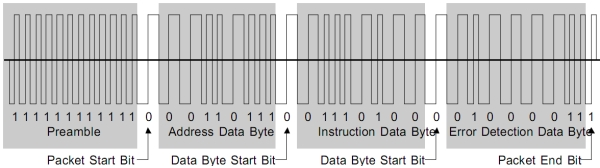
\includegraphics[scale=0.75]{trame.png}
\caption{Exemple d'une trame DCC}
\label{fig1}
\end{figure}

Ce protocole est un protocole standardis\'e qui permet de communiquer
entre la carte~\emph{FPGA} et les diff\'erents trains et
équipements de voies.
Il utilise une suite de commandes envoy\'ees sur les rails
jusqu'aux diff\'erents trains et composants qui agissent en fonction de
la commande qu'ils reçoivent.
La locomotive peut recevoir \'enormément de commandes différentes,
klaxon, annonces d'entr\'ee de gare, phares...(voir datasheet
locomotive). Elles ne seront pas toutes implement\'ees ici, mais
pourront \^etre rajout\'ees ult\'erieurement. 


\subsection{\underline{Le système d'enclenchement}}
\label{sec:log_ixl}

Le chapitre 2 du document \cite{sun2015} présente un système
ferroviaire. Un système ferroviaire est compos\'e de plusieurs systèmes~:
\begin{itemize}
  \item Les \'equipements de voie (rails, aiguillages...) et les
    trains. C'est la partie visible des passagers. 
  \item Le Poste de Commande ferroviaire qui permet à un \emph{op\'erateur} de
    visualiser, en temps r\'eel, l'\'etat du système (position des trains,
    position des aiguilles...)
  \item Le système d'enclenchement qui assure la s\'ecurit\'e du système
    ferroviaire. Il est plac\'e entre le Poste de Commande ferroviaire
    et les \'equipements de voie. Il interdit les commandes lorsque les
    conditions sont incompatibles avec la s\'ecurit\'e. 
\end{itemize}

La figure suivante pr\'esente les relations entre les diff\'erents
systèmes.\emph{(voir fig~\ref{fig3})}

\begin{figure}[h]
\centering
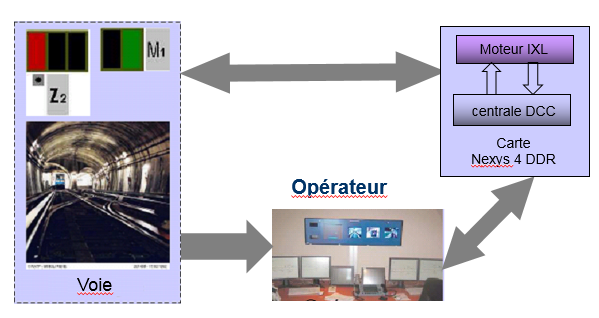
\includegraphics[scale=0.50]{sys_ferro.png}
\caption{Relation entre les différents systèmes}
\label{fig3}
\end{figure}

Un système d'enclenchement est initialement un système réalisé à base
d'un système de clenches (voir figure \ref{clenche}), puis de relais
mécanique (voir figure \ref{relais}). Lorsque les systèmes
d'enclenchement se sont 
informatisés, les relais ont été remplacés par des équations
booléennes (\cite{nyct2016}). Les équations booléennes sont basées sur
les mêmes principes que les relais.

\begin{figure}[ht]
    \begin{minipage}[c]{.46\linewidth}
        \centering
        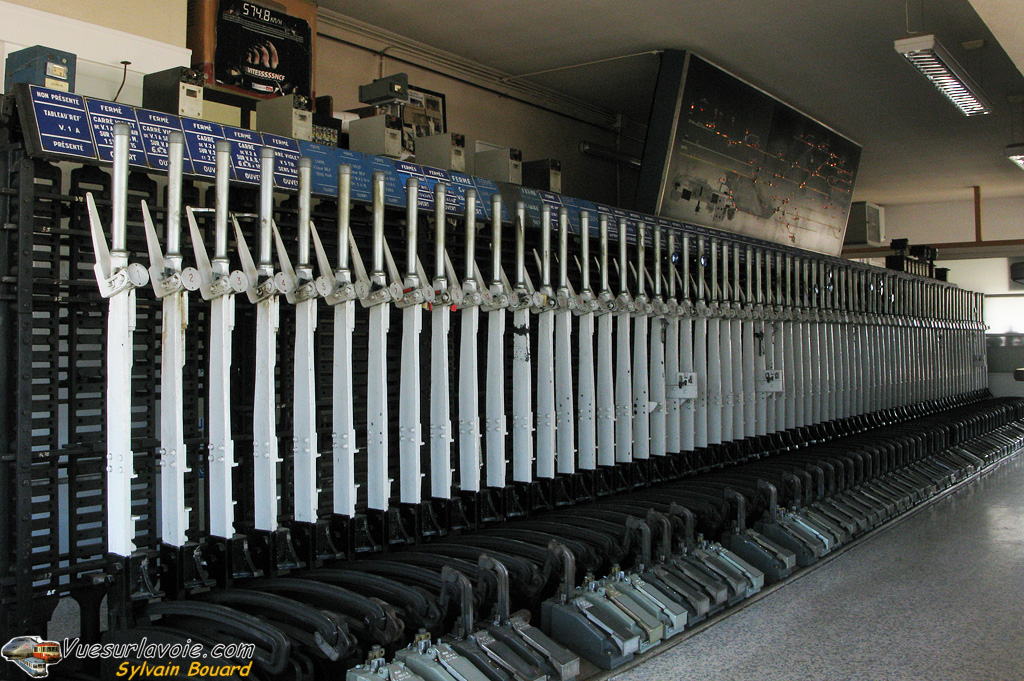
\includegraphics[scale=0.5]{enclenchement_mecanique.jpg}
        \caption{Enclenchement mécanique}
        \label{clenche}
    \end{minipage}
    \hfill%
    \begin{minipage}[c]{.46\linewidth}
        \centering
        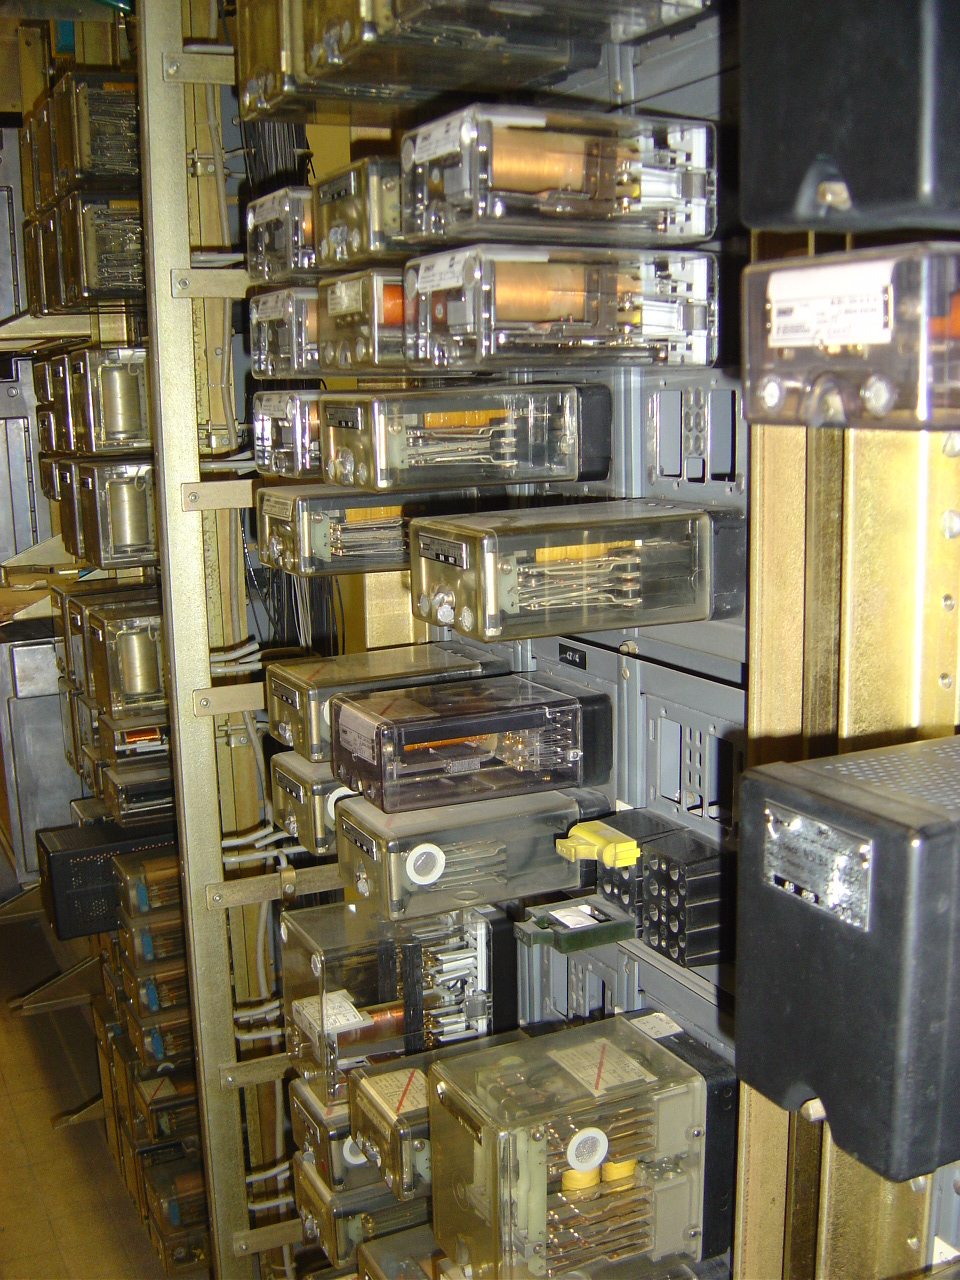
\includegraphics[scale=0.15]{enclenchement_relais.jpg}
        \caption{Enclenchement à relais}
        \label{relais}
    \end{minipage}
\end{figure}


La coeur de la gestion
  ferroviaire est la notion d'\emph{itinéraire} \cite{siteferro}. Un itinéraire
  représente la route entre 2 signaux\emph{(feu)}. Il contient les mouvements
  d'aiguilles nécessaires pour que le train parcourt le chemin entre le
  signal de départ et le signal d'arrivée. Le circuit ferroviaire ne
  contient pas de signaux, ils seront remplacés par des commandes de
  train. Un itinéraire peut être dans les états suivants:
  \begin{itemize}
    \item \emph{commandé}. L'opérateur demande au train de parcourir
      l'itinéraire choisi. Il a par conséquent demandé la formation de
      l'itinéraire au système d'enclenchement. Si les conditions sur
      les aiguilles à manoeuvrer pour former l'itinéraire sont
      correctes, le système d'enclenchement passe à l'état de formation de
      l'itinéraire sinon il est rejeté.
    \item \emph{formé}. Les aiguilles sont positionnées dans la bonne
      direction. Il n'est plus possible de bouger les aiguilles tant
      que le train se situe dans une certaine zone.
    \item \emph{détruit}. Le train a parcouru l'itinéraire, celui-ci peut
      être détruit de façon à autoriser le parcours d'un autre train sur les
      aiguilles.  
  \end{itemize}



Un système d'enclenchement est composé d'enclenchements correspondant
chacun à une condition à vérifier. Par exemple, l'{enclenchement
d'approche d'une aiguille}; Il interdit la formation d'un 
nouvel itinéraire si un train se situe dans la "zone d'approche".
En effet, dans cette zone, un train
n'aurait pas la distance suffisante pour s'arrêter normalement devant
l'aiguille.  Sans cet enclenchement, l'opérateur pourrait détruire
l'itinéraire et commander un autre itinéraire. Le train, ne pouvant
s'arrêter correctement, arriverait sur une aiguille encore en
mouvement et déraillerait.
Sur la figure \ref{encl_approche}, lorsque le train se situe dans la
zone verte, il est possible de bouger l'aiguille A4. Si le train se
trouve dans le zone rouge, alors l'aiguille A4 est \emph{enclenchée}
et toute demande de mouvement de l'aiguille sera rejeté.

%\begin{figure}[h!]
%\centering
%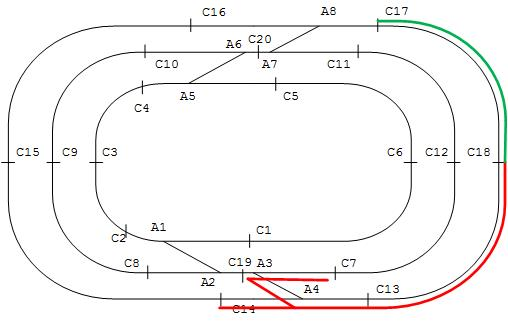
\includegraphics[scale=0.7]{zone_approche.jpg}
%\caption{Enclenchement d'approche d'aiguille}
%\label{encl_approche}
%\end{figure}

\begin{center}
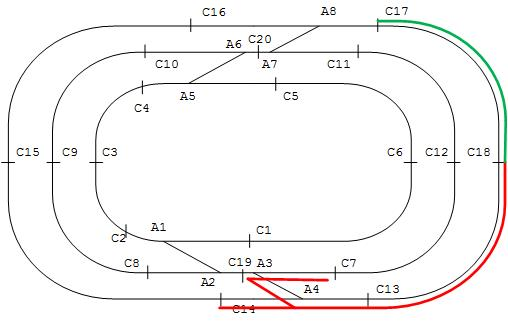
\includegraphics[scale=0.7]{zone_approche.jpg}
\captionof{figure}{Enclenchement d'approche d'aiguille}
\label{encl_approche}%
\end{center}

  
La figure~\ref{archi} présente l'architecture retenue pour le
projet. Elle est composée de 3 parties~:
  \begin{itemize}
    \item La centrale DCC. Elle gère les Entrées/Sorties avec les
      équipements de voie et avec l'IHM. Elle fournit, à la logique
      d'enclenchement, l'état des commandes IHM et des équipements de
      voie et commande les trains. Ceci permet de séparer complètement
      la logique d'enclenchement, de la gestion informatique des
      Entrées/Sorties.
    \item La logique d'enclenchement. Elle contient les équations
      booléennes au format VHDL. 
    \item Le moteur d'instanciation. Il permet de générer, hors temps réel,
      la logique d'enclenchement au format VHDL à partir des équations
      booléennes.
  \end{itemize}

\begin{figure}[ht]
\centering
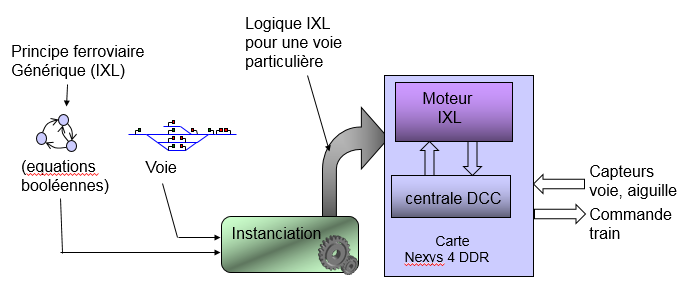
\includegraphics[scale=1]{moteur.png}
\caption{Architecture du projet}
\label{archi}
\end{figure}

Le moteur DCC sera développé en VHDL. Le moteur d'instanciation sera
développé en OCaml \cite{OCAML}.


\newpage
\subsection{\underline{Architecture g\'en\'erale du circuit de train}}
\label{sec:archi}

Voici le sch\'ema repr\'esentant l'installation ferroviaire utilis\'ee
tout au long du projet. 

\begin{figure}[h]
\centering
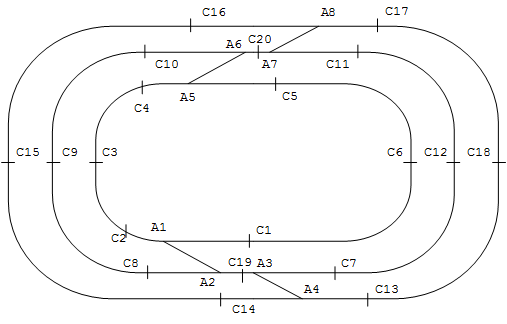
\includegraphics[scale=0.80]{circuit.png}
\caption{Sch\'ema de l'installation}
\label{fig4}
\end{figure}

L'installation \emph{(voir fig~\ref{fig4})} est compos\'ee de 3
circuits imbriqués, de 4 paires d'aiguillages control\'ees par 8
contr\^oleurs gérés par trame DCC, et de 20 capteurs.
Le dispositif peut accueillir jusqu'\`a 6 trains en m\^eme temps.

\begin{figure}[h]
\centering
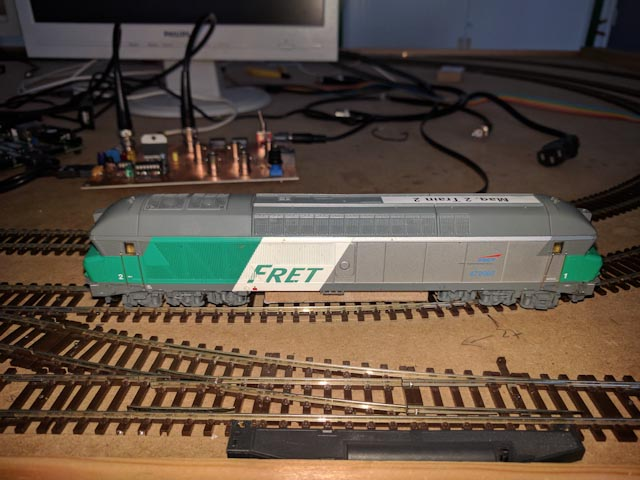
\includegraphics[scale=0.3]{loco.jpg}
\caption{Photo d'une locomotive}
\label{fig5}
\end{figure}

\newpage

Chaque locomotive poss\`ede une adresse sous forme de \emph{code
barre} sous elle \emph{(voir fig~\ref{fig6})}.

Le code barre est compos\'e de la façon suivante :
\begin{itemize}
    \item \textbf{un pr\'eambule} compos\'e de 2 bandes noires
      s\'epar\'ees par 1 bande blanche.
    \item \textbf{de l'adresse} le nombre de bandes noires correspond
      à l'adresse du train. 
    \item \textbf{un \'epilogue} compos\'e de 3 bandes noires
      s\'epar\'ees par 2 bandes blanches.
\end{itemize}

\begin{figure}[h]
\centering
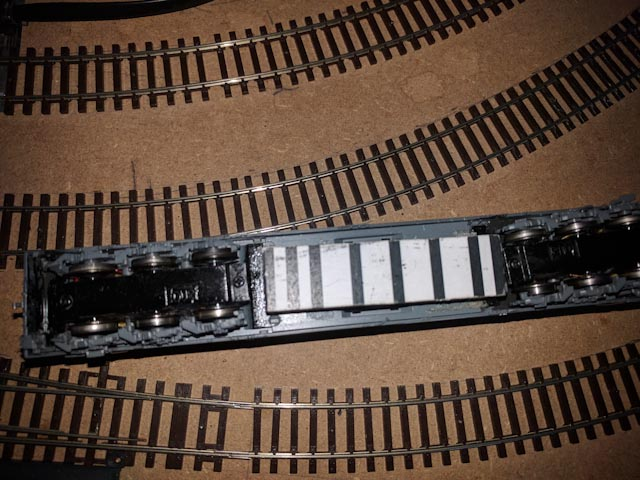
\includegraphics[scale=0.3]{add.jpg}
\caption{Photo de l'adresse sous la locomotive}
\label{fig6}
\end{figure}


L'aiguillage lui est géré par trame DCC, c'est à dire que chaque
contrôleur d'aiguillage possède une adresse qui lui permet de recevoir
une trame contenant une instruction qui lui demande de bouger ou non
l'aiguille.
Cette instruction est donnée sur 2 bits. Et l'aiguille possède deux
états, gauche ou droit, mais ne possède pas d'état intermédiaire.
\newline
\newline
Il y aura plusieurs \emph{itinéraires} prédefinis pour les trains. Un
itinéraire correspond au trajet que l'on veut qu'il effectue, aller
d'une voie ``A`` à une voie ``B`` en passant par exemple par la voie
``C`` en utilisant des aiguillages choisi à l'avance.
\newline
\newline
Les capteurs vont permettre de mettre à jour une table contenant la
dernière position connue de chaque train ce qui va nous permettre de
choisir si un train doit changer de voie ou rester sur la sienne selon
si il y a un train qui bloque ou non la zone d'aiguillage qui nous concerne.

\newpage

\subsection{\underline{Outils}}
\label{sec:outils}

Lors de ce projet, je vais utiliser diff\'erents outils :
\begin{itemize}
  \item La carte \crt comme plateforme de d\'eveloppement
  \item La locomotive \emph{Jouef ``Fret SNCF``}\cite{Jouef}, les capteurs de
    position et des aiguillages
  \item Le protocole DCC \cite{DCC}
  \item Le logiciel Vivado comme \emph{IDE}
\end{itemize}

ainsi que plusieurs langages:
\begin{itemize}
  \item \emph{VHDL}\cite{VHDL} comme language de description pour mes diff\'erentes
    \emph{IP}
  \item \emph{GIT}\cite{GIT} pour la gestion de configuration des logiciels
  \item \emph{\LaTeX}\cite{LATEX} pour la r\'edaction de la documentation
  \item Le langage \emph{Ocaml}\cite{OCAML} pour la g\'en\'eration de la logique d'enclenchement
\end{itemize}


\section{Organisation du projet}
\label{sec:org_proj}

\subsection{\underline{Activit\'es du projet}}
\label{sec:activ}

Comme dit plus haut \emph{(voir 2.5)} le projet va \^etre decoup\'e en
plusieurs \'etapes diff\'erentes.

\begin{enumerate}[1]
  \item Portage de la centrale DCC
  \begin{itemize}
    \item Dans un premier temps il faut cr\'eer une nouvelle Interface
      Homme Machine
    \item Puis porter le code de l'ancienne centrale DCC et la
      gestion des capteurs
  \end{itemize}

  \item Ajout des aiguillages
  \begin{itemize}
    \item Ajouter la gestion de l'aiguillage
    \item Une fois l'aiguillage cr\'e\'e, il va falloir ajouter la
      gestion des itinéraires avec les différents aiguillages
    \item Puis pouvoir commander un itinéraire
      pour faire changer de voie un train uniquement
      sans aucun controle de s\'ecurit\'e.
    \item Et enfin r\'ealiser les diff\'erents sc\'enarios A.
  \end{itemize}

  
  \item Avec aiguillages et capteurs
    \begin{itemize} 
      \item Maintenant que la gestion de l'aiguillage et
        l'aquisition des différents capteurs sont effectués, je vais pouvoir rajouter
        la s\'ecurit\'e dans le systeme pour le rendre plus s\^ur.
      \item Il faut ajouter un moteur IXL\cite{IXL} qui v\'erifira
        l'\'etat des voies avant de valider l'envoie d'une commande \`a
        un train.
      \item Une fois toutes ces étapes réalisées, je pourrai r\'ealiser les
        diff\'erents sc\'enarios B qui permettront de valider les
        demandes du projet.      
    \end{itemize}
\end{enumerate}



\subsection{\underline{Planning pr\'evisionnel}}
\label{sec:planning}

Voici les différentes t\^aches ainsi que le planning que je compte
respecter pour r\'eussir \`a mener \`a bien mon projet. La
figure~\ref{gantt} pr\'esente le diagramme de Gantt du projet.

\begin{figure}[h]
\centering
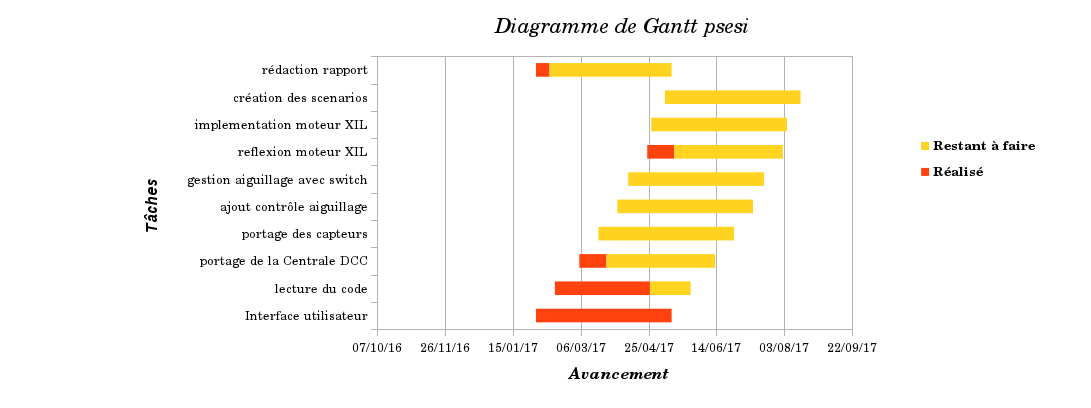
\includegraphics[scale=0.5]{gantt.png}
\caption{Diagramme de Gantt}
\label{gantt}
\end{figure}



\subsection{\underline{Validation}}
\label{sec:valid}

Afin de tester et valider les diff\'erentes \'etapes de mon projet, je vais
faire des \emph{bancs de tests}, des simulations ainsi que des
exp\'erimentations qui pourront permettre de valider les essais.

Il y a d'ailleurs plusieurs sc\'enarios que je vais r\'ealiser qui
me permettront de tester de façon r\'eelle les différents fonctionnements~:


\begin{enumerate}[A]
  \item Sans Capteurs et sans logique d'enclanchement
  \begin{itemize}
    \item 1 train doit passer de la voie ``A`` à la voie ``B``
    \item 2 trains sur la voie ``A``, un seul doit passer sur la voie
       ``B``
  \end{itemize}

\newpage
  
  \item Avec Capteurs et logique enclenchement
  \begin{itemize}
    \item 1 train doit passer de la voie ``A`` à la voie ``B``
    \item 2 trains sur la voie ``A``, un seul doit passer sur la voie ``B``
    \item 1 train 1 sur voie ``A`` qui s'arrête dans la zone aiguillage.
    \item 1 train 2 sur voie ``B``qui veut passer en voie ``A`` --> Pas
       possible. Red\'emarrage train 1, v\'erification du changement de
       voie du train 2.
  \end{itemize}
\end{enumerate}

La première série de tests permettra de valider le fonctionnement de la
centrale DCC. C'est à dire, réception de commandes sur l'IHM, envoi de
commandes aux trains et aux aiguillages. La synchronisation entre les
trains sera faite uniquement sur des temporisations. La logique
d'enclenchement ne sera pas utilisée.

La seconde série de tests permettra de valider la gestion de la sécurité
de la logique d'enclenchement. Elle est basée sur la détection des
capteurs de présence des trains sur la voie. 


\subsection{\underline{Avancement}}
\label{sec:avanc}

J'ai d\'ej\`a commenc\'e \`a travailler sur le projet en essayant de
cr\'eer une IHM pour la s\'election des diff\'erentes commandes que l'on
veut r\'ealiser~:

\begin{itemize}
    \item le choix de \textbf{l'adresse} du \emph{train} qui va
      recevoir la commande
    \item le choix de la \textbf{vitesse} que \emph{le train} s\'electionn\'e
      va recevoir. 
    \item le choix  \textbf{du numéro} de la \emph{route} \`a \'etablir.
    \item les \textbf{features} qui pourront \^etre rajout\'ees au
      projet. 
  \end{itemize}

\newpage

\begin{figure}[h]
    \begin{minipage}[c]{.46\linewidth}
        \centering
        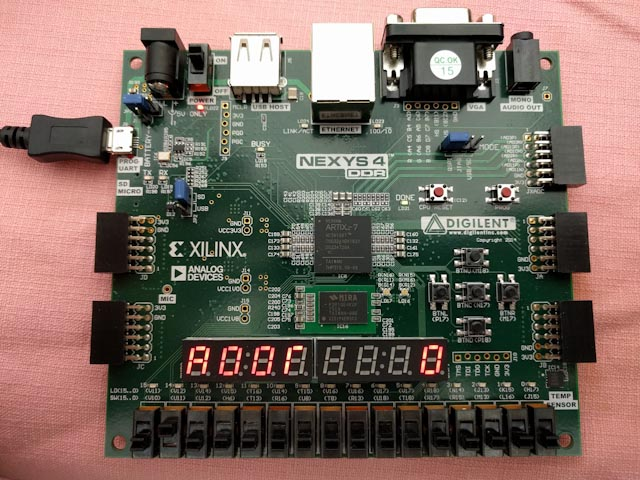
\includegraphics[scale=0.3]{exe_add.jpg}
        \caption{Exemple d'utilisation de la carte}
        \label{carte1}
    \end{minipage}
    \hfill%
    \begin{minipage}[c]{.46\linewidth}
        \centering
        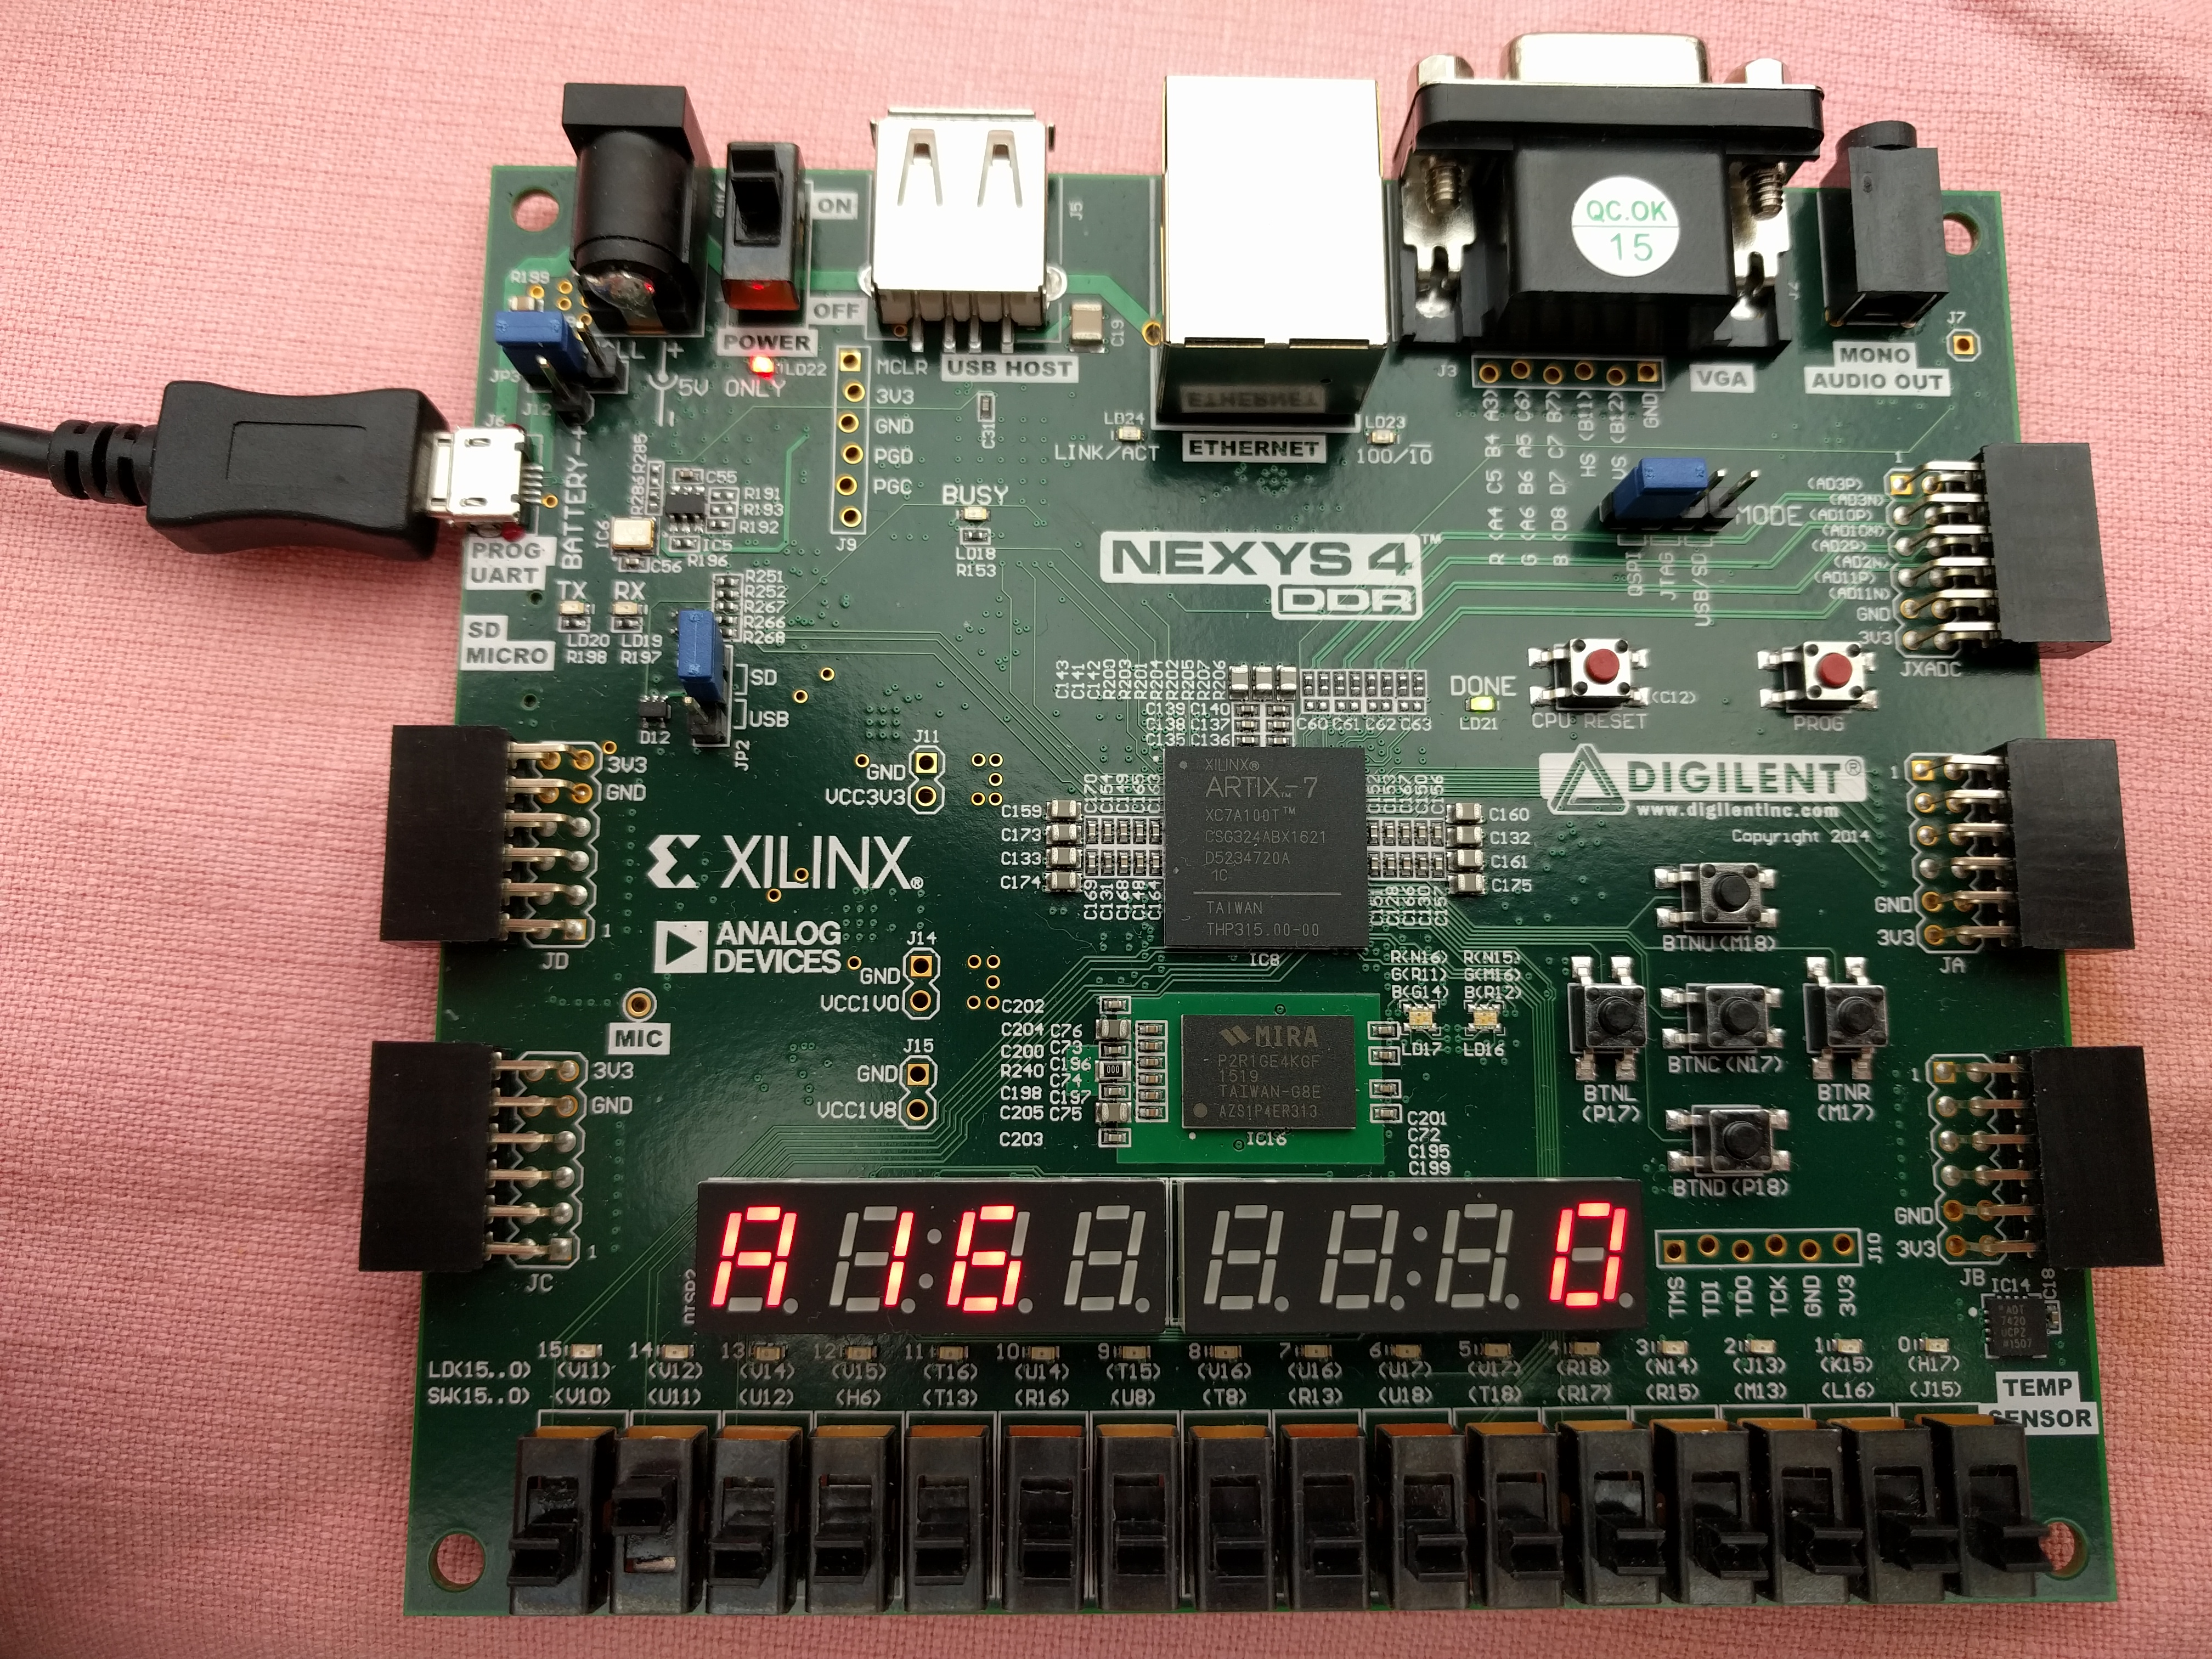
\includegraphics[scale=0.3]{exe_aigui.jpg}
        \caption{Exemple d'utilisation de la carte}
        \label{carte2}
    \end{minipage}
\end{figure}

La \emph{figure~\ref{carte1}} et la \emph{figure~\ref{carte2}} sont un
exemple du rendu de l'IHM d\'evelopp'ee.
La \emph{figure~\ref{carte1}} représente la valeur de l'adresse du
train à qui on envoie la commande.
Tandis que la \emph{figure~\ref{carte2}} montre le numero de
l'aiguillage que l'on veut bouger.
En appuyant sur le bouton gauche on change le réglage, et en appuyant sur le
bouton droit on incrémente la valeur du réglage choisit


Je suis actuellement en train de finir de porter le code de l'ancienne
centrale DCC et de l'aquisition des capteurs sur la nouvelle carte.

\newpage

\bibliographystyle{plain}
\bibliography{biblio}

\end{document}
